%\begin{figure}[t]
    \centering
    \begin{tabular}{m{76mm} m{10mm}} % 2列レイアウト
        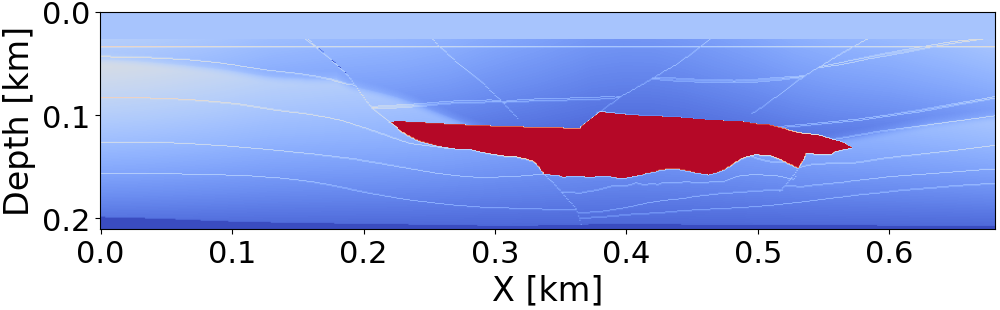
\includegraphics[width=80mm]{public/full_true_vm} &
        \raisebox{1.5mm}{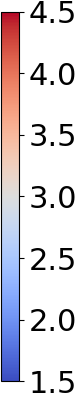
\includegraphics[height=23mm]{public/color-bar}}
    \end{tabular}
    \vspace{-2mm}
    \caption{The velocity model of the Salt [km/s]}
    \vspace{-2mm}
    \label{fig:salt-model}
\end{figure}


We introduce the TV and box constraint into the FWI problem to achieve more accurate reconstruction.
As shown in Fig.~\ref{fig:experiment-data}, the velocity model is piecewise smooth, thus introducing the TV constraint to achieve a more accurate reconstruction.
The box constraint ensures that the velocity model remains within valid ranges.

The optimization problem of the TV and box constrained FWI is formulated as follows:
\begin{equation} \label{eq:FWIObjectiveWithTVConstraint} \argmin{\velModel \in \realNumber^N} \ \ \FWIObjectiveWithTVConstraint \end{equation}
where $\alpha \ge 0$ is the upper bound of the $\ell_{1,2}$ norm, and $u > l > 0$ are the upper and lower bounds of the velocity model values, respectively.
By incorporating TV as a constraint, the parameter $\alpha$ can be determined independently of other terms or constraints, which has been highlighted as an advantage in prior works~\cite{constraint0,constraint1,constraint2,constraint3,constraint4,constraints-vs-penalties-in-FWI}.
This separation makes it possible to directly control smoothness according to $\alpha$, providing a clearer interpretation of the reconstructed subsurface properties.

The constraints can be incorporated into the objective function as indicator functions:
\begin{equation} \label{eq:FWIObjectiveWithTVConstraintWithIndicatorFunction} \argmin{\velModel \in \realNumber^N} \ \ \FWIObjectiveWithTVConstraintWithIndicatorFunction, \end{equation}
where
\begin{equation}
    \label{eq:LOneTwoBallDefinition}
    \begin{aligned}[b]
        \BoxBall & \coloneqq [l,u]^N, \\
        \LOneTwoBall & \coloneqq \LOneTwoBallSetDefinition.
    \end{aligned}
\end{equation}


The proximity operator of $\iota_{\BoxBall}$ and $\iota_{\LOneTwoBall}$ can be computed efficiently.
Therefore, these functions of $E$, $\iota_{\BoxBall}$ and $\iota_{\LOneTwoBall}$ correspond to $f$, $g$ and $h$ in \eqref{eq:PDSPrimalEq}, respectively, $\diffOperator$ is corresponds to $\bm{L}$, so the problem~\eqref{eq:FWIObjectiveWithTVConstraintWithIndicatorFunction} can be solved using PDS.
We show the detailed algorithm in Algorithm~\ref{alg:FWIWithPDS}.
By strictly following the PDS framework, our algorithm accurately solves the optimization problem without relying on approximations or relaxations.
%\begin{equation} \label{eq:FWIWithPDS} \FWIWithPDS \notag \end{equation}
\begin{algorithm}[t]
    \caption{PDS based solver for~\eqref{eq:FWIObjectiveWithTVConstraintWithIndicatorFunction}}\label{alg:FWIWithPDS}
    \begin{algorithmic}[1]
        \Statex \textbf{Input:} $ \velModel^{(0)}, \vecy^{(0)}, \gamma_0 > 0, \gamma_1 > 0 $
        \While {A stopping criterion is not satisfied}
            \State $\widetilde{\velModel} \leftarrow \FWIWithPDSStepMTmp $
            \State $\velModel^{(k+1)}     \leftarrow \FWIWithPDSStepM $
            \State $\widetilde{\vecy}     \leftarrow \FWIWithPDSStepYTmp $
            \State $\vecy^{(k+1)}         \leftarrow \FWIWithPDSStepY $
        \EndWhile
        \Statex \textbf{Output:} $\velModel^{(k)}$
    \end{algorithmic}
\end{algorithm}


The proximity operators of $\iota_{\BoxBall}$, $\iota_{\LOneTwoBall}$, that is, the projection onto $\BoxBall$ and ${\LOneTwoBall}$ are calculated by
\begin{equation} \label{eq:ProximityOperatorForBoxConstraint} \projBoxSolution, \end{equation}
\begin{equation} \label{eq:ProximityOperatorForL12Ball} \projLOneTwoBallSolution \end{equation}
where
\begin{equation} \label{eq:ProximityOperatorForL12BallWhere} \projLOneTwoBallSolutionWhere, \end{equation}
and $\mathfrak{g}_i$ is an index set corresponding to the horizontal and vertical differences of the $i$-th element of $\velModel$.
The proximity operator for the $\ell_1$ norm upper bound constraint is provided in~\cite{L1-ball-projection}.
%The proximity operator for the $l_1$ norm upper bound constraint is expressed as follows~\cite{L1-ball-projection}:
%\begin{equation} \label{eq:ProximityOperatorForL1Ball}  \projLOneBallSolution, \end{equation}
%where
%\begin{equation}
%    \label{eq:ProximityOperatorForL1BallWhere}
%    \begin{aligned}[b]
%        & \bm x_{\text{abs}} = \text{abs}(\vecx), \\
%        & \bm y              = \text{sort}_{\text{desc}}(\vecx_{\text{abs}}), \\
%        & \beta'             = \text{max} \left\{ \frac 1 i \left(\left(\sum_{j=1}^i \bm y_j\right) - \alpha\right) \middle| \ i = 1, \ldots, N \right\}, \\
%        & \beta              = \text{max} \left\{ \beta', 0 \right\}. \\
%    \end{aligned}
%\end{equation}

%\subsection{Computational Cost of Our Algorithm} \label{subsec:computational-cost-of-out-algorithm}
\vspace{2.5mm}
\noindent \textit{Remark}: Computational Cost of Our Algorithm
\vspace{1.5mm}

Our algorithm efficiently solves the optimization problem of the TV and box constrained FWI without relying on inner loops.
Thus, the iteration-dependent factor in the computational cost is eliminated, and the computational complexity to enforce the TV constraint is reduced to $O(N \log N)$, where $N$ is the number of grid points in the velocity model.
Furthermore, existing methods require a computational cost of $O(N \log N)$ or more at each inner-loop iteration, clearly demonstrating the efficiency of our approach.
Due to the reduced cost of incorporating TV constraints, the computational cost at each iteration in our algorithm is dominated by the gradient computation, $\nabla E$, which involves simulating the wave equation along the time axis.
This step has a computational complexity of $O(S\, TN)$, where $S$ is the number of waveform sources and $T$ is the number of time samples.






